\chapter{绪论}
\section{研究背景及意义}
随着空气动力学理论等科学技术的发展,飞行器的速度大幅度提升,对目标进行跟踪探测的精度要求也越来越高,而相应的计算机技术与相关光学理论的日趋成熟也为在飞行器上装载光学探测设备提供了有力支撑,在军事和商业领域通过机载光学设备进行侦察、定位以及识别的工作越来越广泛\cite{huang2008}。特别是在军事领域,在飞行器头部装载具有光学成像功能的目标跟踪、探测以及瞄准光学设备已经成为了目前精确打击武器发展的必然趋势,并且在进行目标跟踪探测的同时对信息获取的精确性以及时效性的要求也大幅度提高\cite{eric2006,shiyipeng2015}。

伴随着这个发展趋势,气动光学问题也应运而生,飞行器在大气中高速飞行时,与大气来流之间由于相互作用会形成结构复杂的流场\cite{busse2004},由于相互作用导致流场中气体的密度会随机变化,使流场的折射率也相应地呈现非均匀性质,这将会影响对目标进行探测的光信号的传输,从而导致成像系统中的目标图像发生偏移、模糊、抖动以及能量的衰减等现象\cite{ejjumper2001},这种效应称为气动光学效应,会严重影响制导的精度。

图\ref{fig:aero}简单展示了来流与飞行器相互作用产生非均匀流场从而引发气动光学效应的产生,当飞行器高速飞行时,其光学头罩与来流发生剧烈的相互作用,头罩温度升高,使光学成像探测系统处于严重的气动热环境。为了减少气动热效应对成像及光学仪器的破坏,一般飞行器都选择在机身侧面装备凸台或凹窗型光学设备,但即便如此,这些光学窗口周围的湍流流场仍然严重影响成像质量,因此有必要对高速流场的运动机理及其对光学传输效应的影响进行研究。
\begin{figure}[hbpt]
\centering
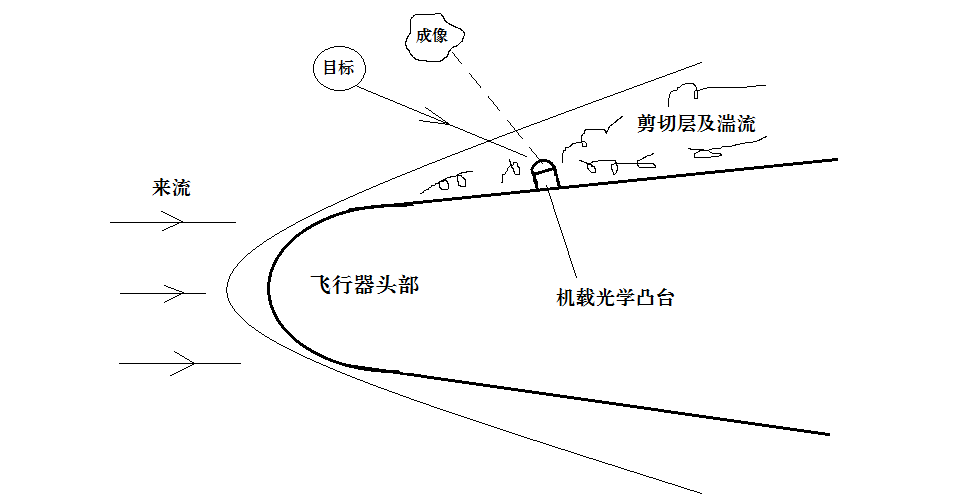
\includegraphics[width=0.8\linewidth]{aerooptic.png}
\caption{气动光学效应示意图}
\label{fig:aero}
\end{figure}

飞行器的速度越快,气动光学效应越明显,成像质量越差,制导精度越低,通过对气动光学效应的机理研究,可以深入分析可压缩流场对光波传输和光学成像的影响,以及研究如何对流场的物理参量进行控制,从而减少这些影响,提高成像质量及跟踪瞄准精度。

飞行器上一般会装备光学凹窗或者凸台来进行目标探测跟踪,由于凸台位于飞行器外侧,信号接收范围较广,因此在飞行器上采用机载凸台光学设备,能够有效扩大目标探测及主动观察寻的范围,同时凸台周围由于受到飞行器前部壁面导致的剪切流影响,并且容易形成二次剪切,这种情况导致凸台周围的流场较为复杂,对光传输影响较大,因此需要对机载凸台周围的流场产生的气动光学效应进行详细研究,从而为精确制导及目标跟踪提供有力支撑。

\section{气动光学的研究进展}
\subsection{气动光学理论的研究进程}
对于湍流的研究可以追溯到1883年,通过将染料喷射到壁面光滑透明的圆管内流体中的实验,英国物理学家Reynolds首次系统地研究层流向湍流的转换过程,发现了两种运动状态具有本质区别并确定了发生条件,他发表于1894年的文章中提出了今后被称为Reynolds数的无量纲参数,当雷诺数大于一个临界值时,流体的扰动不论多小,都将形成剧烈且随机的非常规运动,从而形成湍流\cite{renolds1894}。

而关于湍流对光学传输的影响的研究则要等到1952年,Liepmann采用纹影系统,分析了准直光束通过湍流流场产生的光学像差,首次定性地分析了气动光学像差,并且引入了对气动光学十分重要的均方偏差角的概念\cite{liepman1952}。
并且Baskins和Hamilton也在1952年对超声速湍流流场进行了试验,分析了光波在流场中的传播规律\cite{baskins1952}。

Stine等人于1956年成功地实现了焦平面上对时间平均辐射场的光学测量,他们主要利用初始平面光波通过针孔$(\Phi0.02\text{mm}\sim\Phi0.8\text{mm})$的方法进行测量\cite{stine1956},验证了Liepmann提出的偏差角公式,分析了流场中的电磁波散射情况,并且在参考前人工作的基础之上作了相对成熟的湍流场中的散射情况研究\cite{tatarski1961,villars1954,booker1950},Stine等人的工作为采用光学测量的研究方法来推演湍流的涡旋尺度提供了一定的参考价值,并且这种通过光学的信号测量来反向推测流场尺度特征的方法在今后成为了研究气动光学效应的一种重要研究手段。
 
G.W.Sutton在1969年的研究报告从理论上研究了湍流产生的折射率脉动对光束传播的影响,并且建立了基于物理光学的研究气动光学效应的数值模拟模拟方法,第一次提出相位变化作为评价指标,将远场成像的光斑光强分布情况和近场的波面畸变联系在一起,同时耦合了湍流对光强的衰减系数、相位均方差等,为今后的理论研究打下了夯实的基础\cite{sutton1969},Sutton的工作对于气动光学的研究具有里程碑式的意义,在1985年,他再次作了相关内容的报告,总结了之前关于气动光学的研究主要处于光学试验测量方法的研究阶段,指出下一个阶段的研究应该将重点放在具有实用价值的光学凹窗或凸台附近湍流流场的气动光学研究上\cite{sutton1985}。
 
美国航空航天局于1982年发表的综述\cite{gilbert1982}性文章比较详细地介绍了一些气动光学相关研究方法,包括基于时间平均流场的光波相位畸变$\sigma^2_\Phi$的数值计算方法以及一些比较基本的光学测量手段,比如阴影法和干涉法等直接测量方法,同时也介绍了使用间接测量的方法测量流场的速度以及流场密度,指出了对边界层研究的重要性\cite{trollinger1982}。

二十世纪九十年代,人们进行了很多对相位变化进行计算的理论模型,对斯特列尔比及光学传递函数等光场计算手段进行了研究,气动光学的动态测量技术在这个时期得到了迅速发展,华盛顿大学的Y.P.Tsai和W.H.Christiansent在1990年发表的文章指出了改善气动光学效应的方法,他们主要采用二维的欧拉方程来研究分析光束经过流场的剪切层时的传输特性\cite{tsai1990},并且这一结论的正确性得到了华盛顿大学的Larry Chew和WalterChristiansent的具体实验论证\cite{larry1990},证明了欧拉方程分析方法的可行性。

圣母大学的 Eric J. Jumper 和 Ronald J. Hugo在1995年成功地采用小孔径光束技术量化地测量了光波的波前畸变,这项技术是基于Malley探针的基础上实现的,文中指出这种方法可以用来评价湍流对气动光学效应的影响\cite{jumper1995},次年,两人发表了关于该项技术深度分析的论文\cite{hugo1996},文中指明这种测量方法可以用于测量湍流随机脉动的频率、当地速度以及湍流的脉动尺度等,他们积极地推广了小孔径光束测量技术,并且在此之后圣母大学通过这项技术在气动光学的研究中发挥了积极的作用, 2000年,两人再度合作发表的论文中构建了通过折射率场计算光波相位差的简化方程,并且该方程的可靠性已经经过了具体试验的验证\cite{hugo2000}。

在二十一世纪初期,关于气动光学理论的研究主要集中在具体湍流流场的机理研究以及光学方面的理论研究、测量方法上,美国圣母大学的Jumper与波音公司的Fitzgeraldb 两人合作完成了在这个时期的一项里程碑似的工作,他们发表的文章\cite{jumper2001}对该时期气动光学研究的特点进行了详细综述,文中主要介绍了气动光学研究的实验和测量技术的方法以及在实际应用领域中的发展情况,并且回顾了启动光学研究至今的发展历程,预测了在不远的将来,飞行器上将会装载高效可用的光学探测设备。 

Michael在2010年成功地利用高阶抛物方程近似求解气动光学效应,文中证明出采用四阶龙格-库塔配合第二阶的方法求解时拥有很高的精度,并且可以用高阶拉格朗日插值再度提高准确性\cite{michael2010},并且文中发现波长较短的光束在通过湍流区域时拥有更好的聚拢性,在计算中使用短波也更加精确。

Meng Wang等人在2012年的文章再次系统性地回顾了关于湍流介质引起的光学畸变现象的研究,重点介绍了气动光学的数值计算预测和物理机制\cite{meng2012}。文中提出,经过一系列流场包括湍流边界层、分离剪切层和光学设备周围的湍流的研究,通过数值模拟和实验研究,对这些现象有了一些新的物理理解。指出目前的核心问题在于可压缩湍流有较大的不确定性,并且大多数研究停留在亚音速阶段,提出需要更加精确的实验和计算技术来预测湍流运动,并简要讨论了削弱气动光学效应的方法。

国外的科学家们对气动光学的理论研究已经比较深入,发展了多种计算模型并且对湍流的运动机理进行了比较成熟的理论分析,但是目前较多的研究停留于低音速阶段,对于超音速的流场研究较少,且计算精度有待提高。
\subsection{实验及数值模拟上的进展}
气动光学问题是由于高速飞行器周围流场对目标成像及制导的严重影响而提出的,因此,早期的研究热点大都是以工程实用为目的的试验研究,美国、俄罗斯等大国对此投入了大量的成本,成立了专门的研究机构并建立相应的试验场地和实验设备等以展开长期深入的研究,并且研发了很多针对气动光学效应的数值计算分析的软件,在削弱气动光学效应方面取得了重要进展。

由于气动光学效应主要是高速飞行的飞行器周围流场导致的,因此对于气动光学效应的实验研究需要基于高速流场来研究,目前来说主要可以通过风洞来模拟具体的流场情况,例如阿诺德工程发展中心(AEDC)建立的高超声速风洞,如图\ref{fig:fengdong},它主要用来从事气动光学机理的实验验证工作\cite{havener1992},在二十世纪末,该工程中心9号风洞就能够在6s内完成流场结构及其引起的波面畸变的同时测量。基于对高超声速飞行器周围流场的实验研究需求,美国在上世纪八十年代建立了国家高能激波风洞,该风洞的两套设备能够提供2至15马赫数的流体速度,并且在后期对其进行了改造,使之能够满足气动光学在试验上的验证研究工作\cite{claspan1990}。
\begin{figure}[bhtp]
\centering
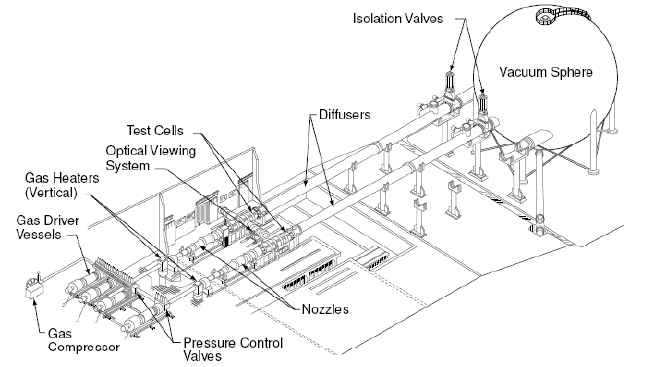
\includegraphics[width=0.9\linewidth]{fengdongshiyan.PNG}
\caption{阿诺德工程发展中心9号风洞机理图}
\label{fig:fengdong}
\end{figure}

近年来,气动光学的研究由大量的实验研究拓展到实验和数值模拟同时进行上,研究重点依然为气动光学效应机理研究以及对机载光学设备气动光学效应的控制。

Stanislav Gordeyev 和 Eric J. Jumper于2003年在实验中使用之前提出的小孔径光束技术研究了湍流边界层中的气动光学特性,实验研究的结果发现目标图像畸变程度与来流的速度的平方、来流密度以及湍流边界的层厚度存在正比例关系\cite{stanislav2003}。

Roberto C. Aguirre 和 Haris J. Catrakis在2004年为了分析当地尺度的波前特征,提出了一种气动光学波前各向异性参数的概念,并发展了基于该各向异性参数的气动光学评价方法\cite{aguirre2004},发现各向异性参数的可以用来衡量湍流引起的波前尺度的特性,当参数等于某一特定值时,光波波前在一定的小范围内拥有自仿射的特性。

Mani 和 Ali 等人在2005年采用大涡模拟的方法,研究了圆柱形的湍流流场对不同波长的光波产生的成像影响\cite{mani2005},发现波长较短的光束的远场成像主要受小涡旋影响。

John E. Pond 和 George W. Sutton在2006年采用三维流体运动方程组结合标准$k - $\textepsilon 湍流模型的数值计算方法,对三维凸台周围的流场进行了数值模拟,采用相位差和斯特列尔比两种参数对气动光学效应进行了评价,文中指出,可光学可调节的适应性系统虽然能够适当地减弱时间平均流场产生的气动光学效应,但是对脉动的湍流流场的矫正效果并不大\cite{john2006}。

Eric Tromeur 和 Eric Garnier在2006年为了求解光束通过流场时产生的相位差,采用了大涡模拟以及利用Sutton 模型分别与雷诺平均法和大涡模拟结合的三种方法对光束经过湍流流场后的相位变化进行求解\cite{tromeur2006},文中结果指出采用大涡模拟直接模拟流场,求解出的光学相位差有最高的精度,并且指出 Sutton的模型应用在非平衡边界层中时,求解得到的气动光学相位差有较大的误差。

2008年,Aaron P. Freeman 和 Haris J. Catrakis尝试了在湍流中注入不同频率的等离子体,证明了这种方法可以用来削弱气动光学效应\cite{freeman2008},成功地减少了27\%的光程差均方根。

Wyckham C 等人在2009年对流场产生的气动光学畸变进行了研究,主要将氦气射入从低音速到高超声速等不同速度的流场中,对光束经过其边界层后产生的光学畸变进行对比,得出了光学畸变主要是由于流场中的大尺度结构决定的,从而证明了大孔径近似理论的正确性\cite{wyckham2006}。

气动光学效应的风洞实验条件比较苛刻,并且实验成本较高、研究周期较长,而随着计算机技术的飞速发展,采用理论模型对流场进行数值模拟已经成为可能,并且相对于风洞实验能够有效节省成本,同时可以对流场参数进行调节从而控制流场结构并多次重复模拟,因此采用数值模拟的方法研究气动光学效应可以快速准确地给出精确结果,经过多次模拟达到预期效果后可以通过风洞试验进行验证。
\section{国内研究现状} 
国内关于气动光学的研究起步比较晚,在二十世纪末,中国航天科工集团提出了气动光学研究是高速导弹发展的重要组成部分,自此,国内的气动光学研究主要以工程需求带动基础研究,
随后的几年时间中航天科工集团多次发表了相关文章,对于国内在气动光学问题的研究成果进行了详细介绍,大大推进了中国气动光学的研究。随后,国内对气动光学效应的理论及实验研究、数值模拟、校正方法等方面都有一定成就,尤其是殷兴良和李桂春两位学者的研究气动光学的专著,对中国研究超声速飞行器光学头罩周围湍流流场的气动光学效应有非常重要的指导作用\cite{deng2008}。

2003年,殷兴良先生撰写了中国国内第一部研究气动光学的专著《气动光学原理》,中国工程院院士并且身为我国光学事业奠基人的王大珩先生称赞这本专著是“建立了国内该领域研究的基础”,以及“标志着我国气动光学这门现代光学新分支学科的形成”\cite{yxl2003qdgxyl},该书分为三个篇章,分别为气动光学研究的数理基础、描述及矫正方法的探讨,总结概括了中国航天二院下属的气动光学课题研究组多年以来的研究成果,对国内学者关于气动光学方面的科研工作提供了重要帮助,促进了我国气动光学的发展。

2006年,李桂春的《气动光学》正式出版,这本书被中国科学院院士庄逢甘先生评价为“将带动相关学科跨越式发展,拓展学科的研究领域,对国民经济建设及现代化建设具有实际的工程应用价值”\cite{liguichun2006}。该书抓住了交叉学科的关键,深入讨论了光波在非均匀介质即气体折射率梯度场$(\nabla n)$和散射场$(\nabla^2 n)$中传输的基本原理,总结了风洞试验中的光学测量技术,填补了国内气动光学学科方面的空白,同样对中国的气动光学发展具有重要意义。

在国内气动光学研究初期,许多学者也发表了大量研究论文,对国内气动光学的研究做出了巨大贡献,例如
郭永洪、 沈忙作等人在1998年的论文中简要介绍了采用数值模拟研究超声速光学头罩气动光学效应的分析过程,分别讨论了平均、湍流流场的气动光学效应以及两者的合成气动光学效应的计算方法\cite{gyh1998}。
费锦东\cite{fjd1998}在1998年发表于红外与激光工程的文章首次指出,由于气动光学效应的存在,高速导弹的红外成像制导系统对于目标的成像清晰度大大降低,提出气动光学效应的校正对于高速导弹光学头罩的外型设计、提高制导的精度以及抗干扰能力具有重要的作用。
房建成,杨照华等在2004年的文章中基于折射率场分别对不同尺度的涡旋结构的光传输特性进行了模型的建立,文中主要利用光线追迹法建立大尺度模型,而用统计光学法建立小尺度涡结构的光学传输模型\cite{fjc2004}。

最近十年,国内关于气动光学的研究得到飞速发展,取得了非常不错的成绩\cite{xie2007}。殷兴良在2006年建立了流场光学的工程计算模型,描述了气动光学效应对光学探测系统影响的经验模型,通过数值仿真,分析了气动光学效应对光学探测系统的影响与飞行器的飞行参数、光学探测系统参数和探测器积分时间的关系\cite{yxl2006gsfxq}。
赵剡等人在2008年的两篇文章基于数值模拟建立了光传输模型对光程差与光程进行了处理,利用带像差的光学传递函数理论,研究了对图像复原的方法\cite{zhao2008,zhaoz2008}。
史可天等人在2010年使用瞄视误差、Strehl 比以及含能半径等光学参数描述了湍流流场引起的光学畸变,具体分析了不同飞行状态和光学参数对光传输的影响\cite{skt2010}。

李波在2011年提出了实现了高速流场的气动光学研究的数值模拟,提出从流场角度出发评估高速流场导致的气动光学性能的评价方法,并且完成了高速飞行器光学窗口的初步设计\cite{libo2011}。
冯定华等人在2012年在通过数值计算得到精确的流场物理参数的基础上,分析了凹腔剪切层的光学传输效应,发现气流的剪切层结构会使光线抖动从而导致波面畸变,从而减少了斯特列尔比,削弱光束强度,并且会导致图像的位移,降低制导精度\cite{fdh2012}。
徐博在2015年利用Matlab及Zemax仿真模拟了对基于随机并行梯度下降算法的像清晰化自适应光学系统,将形镜形状变化引起的光线偏折以及光学系统自身的像差纳入考虑范围,对波前畸变进行了光电校正\cite{xubo2015}。
 
国内关于气动光学的研究已经取得了一定的进展,李桂春以及殷兴良的两部专著对国内关于气动光学理论研究以及光学校正作出了巨大的贡献\cite{yang2009,li2011},并且最近十年的相关研究也取得了飞速突破,同时国内的研究大多是对于凹腔的气动光学进行研究,并且数值模拟方面主要集中于中低音速流场,关于超音速的流场气动光学研究较少。
\section{论文主要研究内容及论文组织架构}
本文的研究来源于航天科技创新基金(SAST201350),国内现阶段对于气动光学效应的研究大多数处于低音速至低超音速流场的阶段,并且光学窗口的研究类型主要为凹窗型的探测窗口,而随着飞行器飞行速度的迅速提升以及探测范围的需求增大,未来精确制导及目标探测领域将集中于高速流场,同时将会装载光学凸台进行大范围的精确探测,因此本文将对高速飞行器和光学凸台周围流场的气动光学效应进行研究,主要研究内容可以分为如下的流场运动和光学传输两大研究方面:

(1)基于流体力学理论,研究从亚音速到高超音速等不同速度下的流场运动机理,讨论流体运动方程组的求解模型以及数值模拟方法,建立有效的数值模拟流程,然后采用计算流体力学(CFD)软件分析高速飞行器及凸台周围流场的情况。

(2)基于物理光学、线性光学、波动光学以及统计光学的理论,对高速流场产生的气动光学效应的机理进行研究,分析流场对光束传输影响的计算方法和评价体系,基于流场数值模拟得到的结果,通过Mathematica数值计算,研究分析凸台光学窗口周围混合流场的气动光学效应。

本论文的组织结构如下:

第一章:说明了课题研究的背景,回顾了以往关于气动光学理论研究、实验测量以及数值模拟方面的成果,分析了研究特点以及存在的困难,提出研究凸台周围高速流场引起的气动光学效应的必要性。

第二章:介绍了流体运动的基本理论,分析了大涡模拟以及雷诺平均模拟两种气动光学的数值模拟方法,推导了基于$k-\varepsilon$模型和$k-\omega$模型的SST混合二方程模型,最后分析了高超声速流场的物理特性。

第三章:对高速流场模拟前需要的定解条件以及控制方程的离散作了相应设置及推导,建立了可压缩流场数值模拟的具体流程,最后通过ICEM建模软件建立了三维导弹、机载凸台的模型,使用Fluent基于$k-\omega$SST二方程模型对不同运行速度下导弹及凸台周围的流场分布进行了数值模拟及分析。

第四章:分析了光束在高速湍流场中的传输特性,基于光线追迹法、波动光学以及统计光学的方法对平均流场、湍流脉动流场分别分析,推演了偏移角、斯特列尔比以及光学传递函数等气动光学评价方法。

第五章:通过G-D系数建立密度与折射率的直接关系,讨论了高斯光束以及夫琅禾费衍射现象,最后基于CFD网格离散化求解方法,计算了不同速度、不同入射角下凸台光学窗口周围的波面畸变,对光学孔径内受湍流流场影响的斯特列尔比和光学传递函数作了计算,得到了高斯光束经过流场前后的光斑变化。
 
 第六章:对本论文的工作作了相应的总结,并且对该课题未来的进一步研究进行了展望。
 
 
 